\documentclass[handout]{beamer}

% math packages
\usepackage{amssymb}

% theme
\usetheme{Rochester}
\usecolortheme{dove}
\usefonttheme{default}

% make the title BIG
\setbeamerfont{title}{series=\bfseries,size=\Huge, parent=structure}

% remove the side title header
\setbeamertemplate{headline}{}

%gets rid of bottom navigation bars
\setbeamertemplate{footline}{}

%gets rid of navigation symbols
\setbeamertemplate{navigation symbols}{}

% define "head" commands for transitions
\newcommand{\headone}{\centering \bf \Huge}
\newcommand{\headtwo}{\centering \bf \LARGE}
\newcommand{\headthree}{\centering \bf \Large}

% define a "spaceit" command for spacing between paragraphs
\newcommand{\spaceit}{\vspace{10mm}}

% define a "red" command to make text red.
\newcommand{\red}[1]{\textcolor{red}{#1}}
\newcommand{\blue}[1]{\textcolor{blue}{#1}}


% simply the style of the lists
\setbeamertemplate{itemize items}[default]
\setbeamertemplate{enumerate items}[default]

% increase the default spacing between equations
\setlength{\jot}{5pt}

% custom color for "blockcode"
\usepackage{fancyvrb,color}

\DefineVerbatimEnvironment{blockcode}
  {Verbatim}
  {formatcom=\color{blue}}


\begin{document}
\title{Quantities of Interest}   
\author{Carlisle Rainey} 
\date{} % remove date 

\frame{\titlepage} 

\frame{
\textbf{We know how to get our point estimates and standard errors.} \\\vspace{5mm}

\begin{enumerate}
\item Write down a probability model.
\item Find the probability of the data given the parameters--the likelihood function.
\item Take the log and simplify.
\item Maximize to find the MLE.
	\begin{itemize}
	\item Analytically. (Usually difficult or impossible.)
	\item Numerically. (Usually easier.)
	\end{itemize}
\item Take the inverse of the negative Hessian at the MLE to find the covariance matrix.
\item Take the square root of the diagonal of the covariance matrix to find the standard errors.
\end{enumerate}
}

\begin{frame}[fragile]
\begin{footnotesize}
\begin{blockcode}
> # load libraries
> library(arm)
> 
> # read data
> d <- read.csv("http://crain.co/am-files/data/turnout-small.csv")
> 
> # estimate simple logit model
> m <- glm(vote ~ educate + age + income, 
+          family = binomial, data = d)
> 
> # display results
> display(m, detail = TRUE)
glm(formula = vote ~ educate + age + income, family = binomial, 
    data = d)
            coef.est coef.se z value Pr(>|z|)
(Intercept) -2.92     0.32   -9.16    0.00   
educate      0.18     0.02    8.89    0.00   
age          0.03     0.00    8.44    0.00   
income       0.18     0.03    6.76    0.00   
---
  n = 2000, k = 4
  residual deviance = 2026.9, null deviance = 2266.7 (difference = 239.9)
\end{blockcode}
\end{footnotesize}
\end{frame}

\begin{frame}[fragile]
\begin{Large}
\begin{blockcode}
            coef.est coef.se z value Pr(>|z|)
(Intercept) -2.92     0.32   -9.16    0.00   
educate      0.18     0.02    8.89    0.00   
age          0.03     0.00    8.44    0.00   
income       0.18     0.03    6.76    0.00  
\end{blockcode}
\end{Large}\vspace{8mm}
We've fought so long and hard for these estimates, what do we do with them? We've got sign-and-significance, but that tells us way less than we'd like to know.
\end{frame}

\frame{
In particular, in otherwise ``Republican'' states (GOP-controlled legislatures, 38\% view ACA favorably, and all other variables set at their sample medians), having a Republican governor (as opposed to a Democratic governor) increases the chance of gubernatorial opposition by about 49 [23, 74] percentage points.\\\vspace{5mm}
\red{This would probability be even better if I mentioned the probabilities that we are changing from and to.}
}

\begin{frame}[fragile, plain]
\hspace*{-10mm}
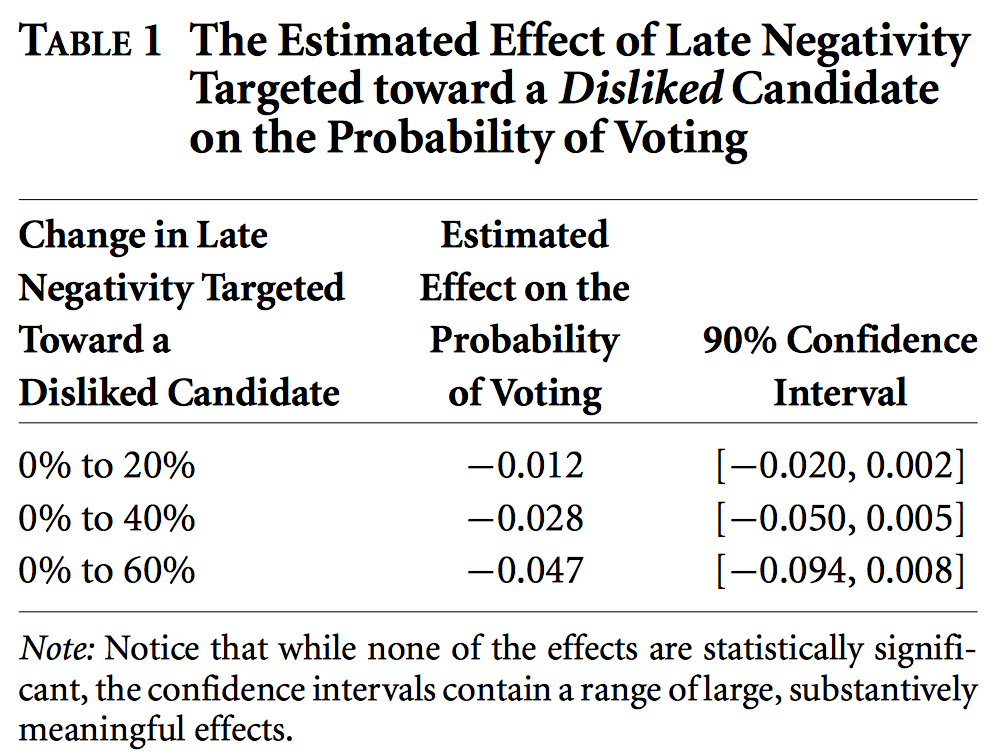
\includegraphics[width=\paperwidth]{figs/nme.png}
\end{frame}

\begin{frame}[fragile, plain]
\hspace*{-10mm}
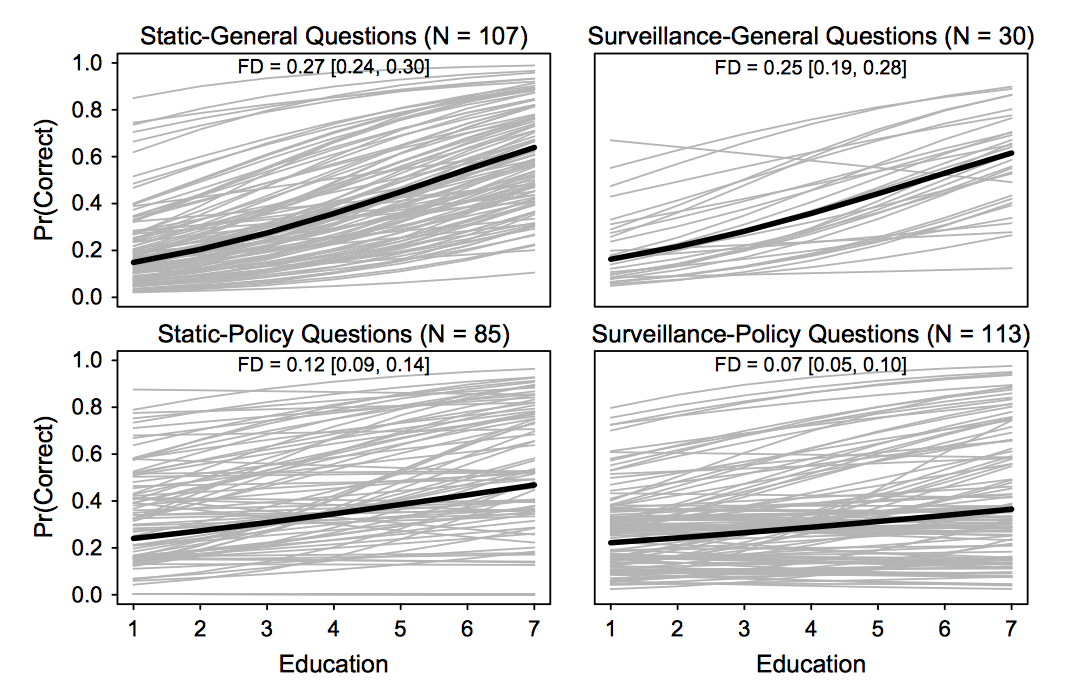
\includegraphics[width=\paperwidth]{figs/quadrants.png}
\end{frame}

\begin{frame}[fragile, plain]
\hspace*{-10mm}
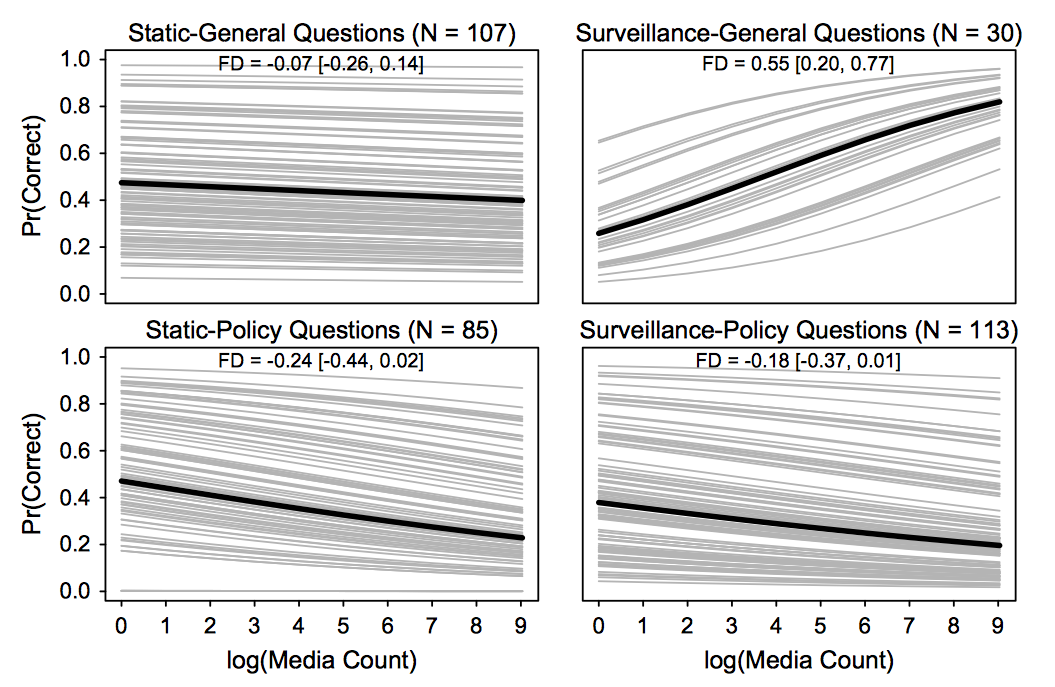
\includegraphics[width=\paperwidth]{figs/quadrants2.png}
\end{frame}

\begin{frame}[fragile, plain]
\hspace*{-10mm}
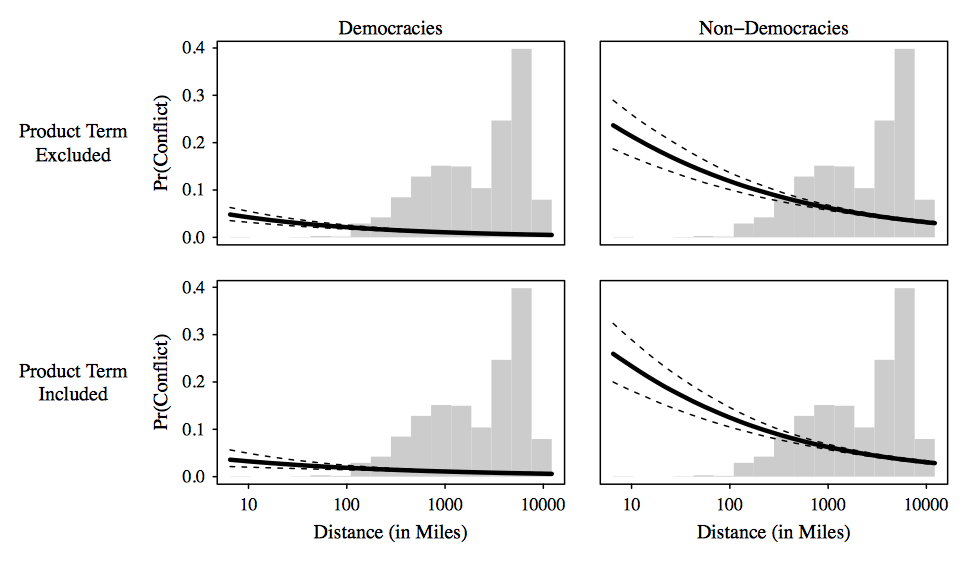
\includegraphics[width=\paperwidth]{figs/compress.png}
\end{frame}

\begin{frame}[fragile, plain]
\hspace*{-10mm}
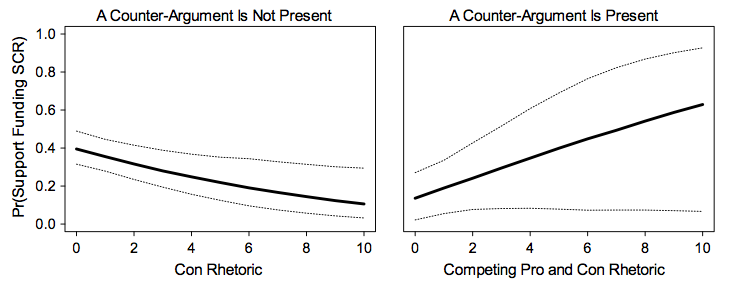
\includegraphics[width=\paperwidth]{figs/rhetoric.png}
\end{frame}

\begin{frame}[fragile, plain]
\hspace*{-10mm}
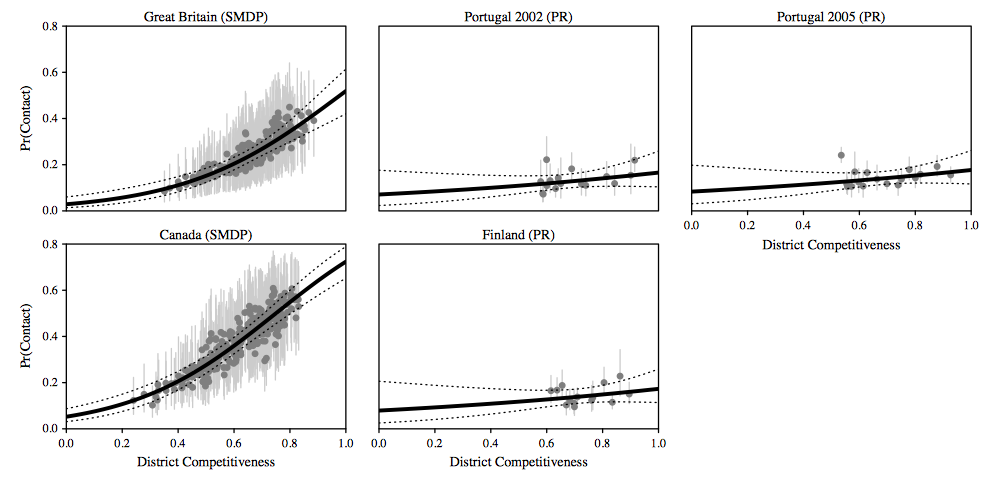
\includegraphics[width=\paperwidth]{figs/stratmob.png}
\end{frame}

\begin{frame}[fragile, plain]
\hspace*{-10mm}
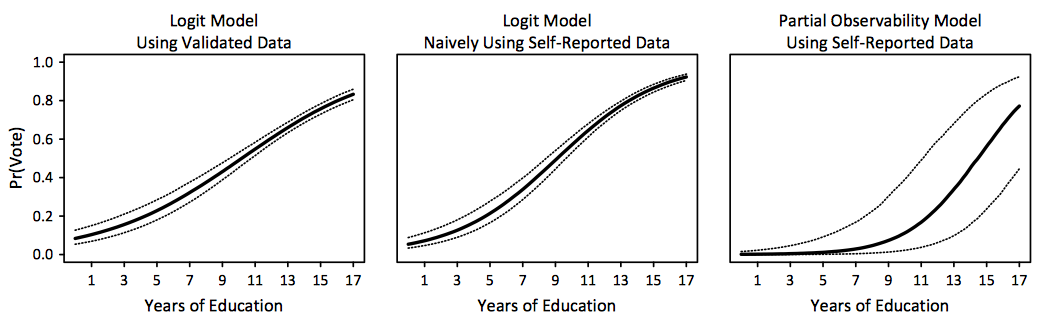
\includegraphics[width=\paperwidth]{figs/unreliable.png}
\end{frame}

\begin{frame}[fragile, plain]
\hspace*{-10mm}
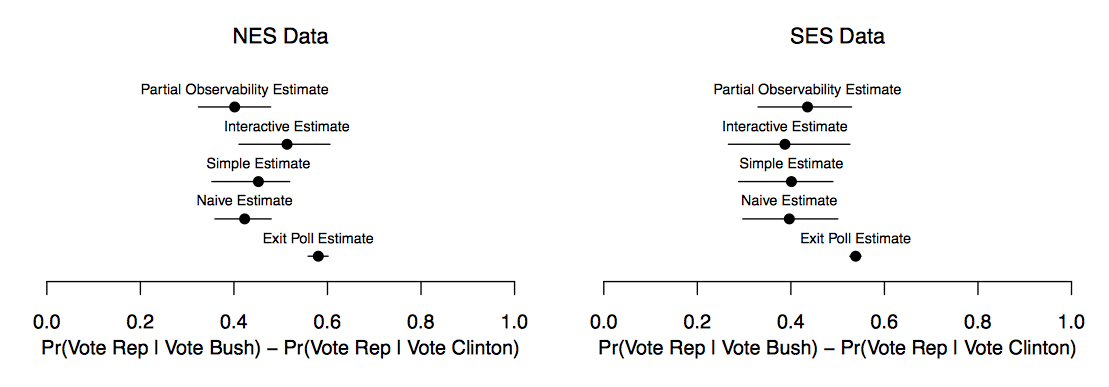
\includegraphics[width=\paperwidth]{figs/misreports.png}
\end{frame}

\frame{
We've talked about point estimates and confidence intervals for coefficients, but we \underline{really} want point estimates and confidence intervals for our \underline{quantities of interest}.\\\vspace{5mm}
We'll do this in two steps:
\begin{enumerate}
\item point estimates (these notes)
\item confidence intervals (the next notes on simulation)
\end{enumerate}
}

\frame{
Theorem (Invariance property of MLEs): If $\hat{\theta}$ is the MLE of $\theta$, then for \underline{any} function $\tau(\theta)$, the MLE of $\tau(\theta)$ is $\tau(\hat{\theta})$.
}

\frame{
A \textbf{quantity of interest} $q(\theta, X_1, X_2,..., X_n)$ is a function of the model parameters and specially chosen ``data sets'' (row-vectors) that are of special substantive interest.\\\vspace{5mm}
This is a very generic definition, let's see some specific examples from the logit model.
\begin{enumerate}
\item predicted probability
\item first-difference
\item risk-ratio
\end{enumerate}
}

\frame{
\textbf{\Large Predicted Probability\footnote{As far as I can tell, there is no reason for the ``predicted.'' We could just say probability. However, everyone always says ``predicted probability'' when talking about this particular quantity of interest. It occasionally leads to some awkward phrasings, but that's okay.}}
\begin{enumerate}
\item Remember, $q(\theta, X_1, X_2,..., X_n)$ in general. 
\item For the logit model, we can replace $\theta$ with $\beta$ to match convention. 
\item For the predicted probability, we just need one specially chosen matrix, which we'll call $X_c$.
\item This leaves $q(\beta, X_c)$.
\item The predicted probability is defined as $q(\beta, X_c) = Pr(y_c) = \text{logit}^{-1}(X_c \beta)$.
\end{enumerate}\vspace{5mm}

For a given values of the covariates $X_c$ and the coefficients $\beta$ what is the probability of an event?
}

\frame{
We have $Pr(y_c) = \text{logit}^{-1}(X_c \beta)$. How can we get the MLE of $Pr(y_c)$, which we might denote as $\widehat{Pr}(y_c)$?\\\vspace{5mm}
\pause We just use the invariance principle--$\widehat{Pr}(y_c) = \text{logit}^{-1}(X_c \hat{\beta})$.\\\vspace{5mm}
\pause Let's see an example.
}

\frame{
\headthree
gist.github.com/carlislerainey\\\vspace{5mm}
\texttt{logit-qi-incomplete-example.R}
}

\begin{frame}[fragile]
\begin{Large}
\begin{blockcode}
            coef.est coef.se z value Pr(>|z|)
(Intercept) -2.92     0.32   -9.16    0.00   
educate      0.18     0.02    8.89    0.00   
age          0.03     0.00    8.44    0.00   
income       0.18     0.03    6.76    0.00  
\end{blockcode}
\end{Large}\vspace{8mm}
{\headthree From these estimates, let's get a predicted probability.}
\end{frame}

\begin{frame}[fragile]
\begin{large}
\begin{blockcode}
# set the medians
x.edu <- median(d$educate)  # in years
x.age <- median(d$age)  # in years
x.inc <- median(d$income)  # in 10,000s of dollars

# set X.c and beta.hat
beta.hat <- coef(m)
X.c <- c(1, x.edu, x.age, x.inc)

# calculate the MLE for the predicted probability
p.hat <- plogis(X.c%*%beta.hat) 
\end{blockcode}
\end{large}
\end{frame}

\frame{
\headone Quantities of Interest\\for Effects\\\vspace{10mm}
}

\frame{
\textbf{\Large First-Difference}
\begin{enumerate}
\item Remember, $q(\theta, X_1, X_2,..., X_n)$ in general. 
\item For the logit model, we can replace $\theta$ with $\beta$ to match convention. 
\item For the first-difference, we need two specially chosen matrices. One matrix will have a particular variable set to an interesting ``high'' value. The other matrix will have the same variable set to an interesting ``low'' value. We'll call these matrices $X_{hi}$ and $X_{lo}$, respectively. All the other variables are set to the same values across $X_{hi}$ and $X_{lo}$.
\item This leaves $q(\beta, X_{hi}, X_{lo})$.
\item The first-difference is defined as 
\begin{equation*}q(\beta, X_{hi}, X_{low}) = FD = \overbrace{\text{logit}^{-1}(X_{hi} \beta)}^{p_{hi}} - \overbrace{\text{logit}^{-1}(X_{lo} \beta)}^{p_{lo}} = p_{hi} - p_{lo}.
\end{equation*}
\end{enumerate}\vspace{5mm}

How does the probability of an event change when $X_{lo}$ changes to $X_{hi}$ for a given $\beta$?
}

\frame{
We have $FD = \text{logit}^{-1}(X_{hi} \beta) - \text{logit}^{-1}(X_{lo} \beta)$. How can we get the MLE of $FD$, which we might denote as $\widehat{FD}$?\\\vspace{5mm}
\pause We just use the invariance principle--$\widehat{FD} = \text{logit}^{-1}(X_{hi} \hat{\beta}) - \text{logit}^{-1}(X_{lo} \hat{\beta})$.\\\vspace{5mm}
\pause Let's see an example.
}

\begin{frame}[fragile]
\begin{large}
\begin{blockcode}
# set the medians
x.edu.lo <- 12  # in years
x.edu.hi <- 16  # in years
x.age <- median(d$age)  # in years
x.inc <- median(d$income)  # in 10,000s of dollars

# set X.hi, X.lo, and beta.hat
beta.hat <- coef(m)
X.lo <- c(1, x.edu.hi, x.age, x.inc)
X.hi <- c(1, x.edu.hi, x.age, x.inc)

# calculate the MLE for the first-difference
p.hi.hat <- plogis(X.hi%*%beta.hat) 
p.lo.hat <- plogis(X.lo%*%beta.hat) 
fd.hat <- p.hi.hat - p.lo.hat
\end{blockcode}
\end{large}
\end{frame}

\frame{
\textbf{\Large Risk-Ratio}
\begin{enumerate}
\item For the risk-ratio, we need two specially chosen matrices, $X_{hi}$ and $X_{lo}$, just like for the first-difference.
\item The risk-ratio is defined as 
\begin{equation*}
q(\beta, X_{hi}, X_{low}) = RR = \dfrac{\text{logit}^{-1}(X_{hi} \beta)}{\text{logit}^{-1}(X_{lo} \beta)} = \dfrac{p_{hi}}{p_{lo}}.
\end{equation*}
\end{enumerate}\vspace{5mm}

How many times more likely is an event under $X_{hi}$ compared to $X_{lo}$ for a given $\beta$?
}

\frame{
We have $RR = \dfrac{\text{logit}^{-1}(X_{hi} \beta)}{\text{logit}^{-1}(X_{lo} \beta)}$. How can we get the MLE of $RR$, which we might denote as $\widehat{RR}$?\\\vspace{5mm}
\pause We just use the invariance principle--$\widehat{RR} = \dfrac{\text{logit}^{-1}(X_{hi} \hat{\beta})}{\text{logit}^{-1}(X_{lo} \hat{\beta})}$.\\\vspace{5mm}
\pause Let's see an example.
}

\begin{frame}[fragile]
\begin{large}
\begin{blockcode}
# calculate the MLE for the first-difference
p.hi.hat <- plogis(X.hi%*%beta.hat) 
p.lo.hat <- plogis(X.lo%*%beta.hat) 
rr.hat <- p.hi.hat/p.lo.hat
\end{blockcode}
\end{large}
\end{frame}

\frame{
\textbf{\Large Marginal Effect}
\begin{enumerate}
\item For the marginal effect, we just need one specially chosen matrix $X_{c}$. This is the marginal effect at a specific \emph{point}.
\item The marginal effect of $x_k$ is defined as $ME = \dfrac{\partial Pr(y_c)}{\partial x_k}$. Let $Pr(y_c) = p_{c}$, and, from the homework, we know that 
\begin{equation*}
ME = \dfrac{\partial Pr(y_c)}{\partial x_k} = \overbrace{F'(X_c\beta)\beta_k}^{\text{chain rule}} = p_c(1 - p_c)\beta_k.
\end{equation*}
\end{enumerate}\vspace{5mm}

What is the instantaneous effect (i.e., slope of the tangent line) of $x_k$ on $Pr(y_c)$ at $X_{c}$ for a given $\beta$?
}

\frame{
We have $ME = p_c(1 - p_c)\beta_k$. How can we get the MLE of $ME$, which we might denote as $\widehat{ME}$?\\\vspace{5mm}
\pause We just use the invariance principle--$\widehat{ME} = \hat{p}_c(1 - \hat{p}_c)\hat{\beta}_k$.\\\vspace{5mm}
\pause Let's see an example.
}

\begin{frame}[fragile]
\begin{large}
\begin{blockcode}
# set the medians
x.edu <- median(d$educate)  # in years
x.age <- median(d$age)  # in years
x.inc <- median(d$income)  # in 10,000s of dollars

# set X.c and beta.hat
beta.hat <- coef(m)
X.c <- c(1, x.edu, x.age, x.inc)

# calculate the MLE for the marginal effect
p.hat <- plogis(X.c%*%beta.hat) 
me.hat <- p.hat*(1 - p.hat)*beta.hat["educate"]
\end{blockcode}
\end{large}
\end{frame}

\frame{
\headone Quantities of Interest\\for Interaction\\\vspace{10mm}
\headthree
How does the effect of one variable change with another?
}

\frame{
\textbf{\Large Cross-Partial Derivative}
\begin{enumerate}
\item For the marginal effect, we just need one specially chosen matrix $X_{c}$. This is the cords-partial derivative at a specific \emph{point}.
\item The cross-partial derivative of $Pr(y_c)$ w.r.t. $x_j$ and $x_k$ is defined as $CPD = \dfrac{\partial^2 Pr(y_c)}{\partial x_j \partial x_k}$. As before, let $Pr(y_c) = p_{c}$, and, from the homework, we could figure out that
\begin{equation*}
CPD = \dfrac{\partial^2 \text{Pr}(y_c)}{\partial x_j \partial x_k} =  p_c(1 - p_c)(1 - 2p_c)\beta_j\beta_k.
\end{equation*}
\end{enumerate}\vspace{5mm}

What is the instantaneous effect of $x_j$ on the instantaneous effect of $x_k$ on $Pr(y_c)$ at $X_{c}$ for a given $\beta$?
}

\begin{frame}[fragile]
\begin{large}
\begin{blockcode}
# set the medians
x.edu <- median(d$educate)  # in years
x.age <- median(d$age)  # in years
x.inc <- median(d$income)  # in 10,000s of dollars

# set X.c and beta.hat
beta.hat <- coef(m)
X.c <- c(1, x.edu, x.age, x.inc)

# calculate the MLE for the cross-partial derivative
p.hat <- plogis(X.c%*%beta.hat) 
cpd.hat <- p.hat*(1 - p.hat)*(1 - 2*p.hat)*
           beta.hat["educate"]*beta.hat["age"]
\end{blockcode}
\end{large}
\end{frame}

\frame{
\textbf{\Large Second-Difference}
\begin{small}
\begin{enumerate}
\item For the second-difference, we need \underline{four} specially chosen matrices. 
	\begin{enumerate}
	\item The first matrix $X_{hi, hi}$ will have $x_j$ and $x_k$ set to ``high'' values. 
  	\item The second matrix $X_{lo, hi}$ will have $x_j$ set to a ``low'' value and $x_k$ set to a ``high'' value. 
  	\item The third matrix $X_{hi, lo}$ will have $x_j$ set to a ``high'' value and $x_k$ set to a ``low'' value. 
	\item The fourth matrix $X_{lo, lo}$ will have $x_j$ and $x_k$ set to ``low'' values. 
	\item All the other variables are set to the same values across $X_{hi}$ and $X_{lo}$.
	\end{enumerate}
\item The second-difference is defined as 
\begin{equation*}
SD = (p_{hi, hi} - p_{lo, hi}) - (p_{hi, lo} - p_{lo, lo})
\end{equation*}
\end{enumerate}\vspace{5mm}
How much bigger is the first-difference of $x_j$ when $x_k = hi$ than when $x_k = lo$?
\end{small}
}

\frame{
We're just rocking the invariance principle again.
}

\begin{frame}[fragile]
\begin{small}
\begin{blockcode}
# set the medians
x.edu.lo <- 12  # in years
x.edu.hi <- 16  # in years
x.age.lo <- 25
x.age.hi <- 75
x.inc <- median(d$income)  # in 10,000s of dollars

# set X.hi, X.lo, and beta.hat
beta.hat <- coef(m)
X.hi.hi <- c(1, x.edu.hi, x.age.hi, x.inc)
X.lo.hi <- c(1, x.edu.lo, x.age.hi, x.inc)
X.hi.lo <- c(1, x.edu.hi, x.age.lo, x.inc)
X.lo.lo <- c(1, x.edu.lo, x.age.lo, x.inc)

# calculate the MLE for the first-difference
p.hi.hi.hat <- plogis(X.hi.hi%*%beta.hat) 
p.lo.hi.hat <- plogis(X.lo.hi%*%beta.hat) 
p.hi.lo.hat <- plogis(X.hi.lo%*%beta.hat) 
p.lo.lo.hat <- plogis(X.lo.lo%*%beta.hat) 
sd.hat <- (p.hi.hi.hat - p.lo.hi.hat) - 
          (p.hi.lo.hat - p.lo.lo.hat) 
\end{blockcode}
\end{small}
\end{frame}

\frame{
In particular, in otherwise ``Republican'' states (GOP-controlled legislatures, 38\% view ACA favorably, and all other variables set at their sample medians), having a Republican governor (as opposed to a Democratic governor) increases the chance of gubernatorial opposition by about 49 [23, 74] percentage points.\\\vspace{5mm}
\red{We know how to get that 49 now. But where does the confidence interval come from?}
}

\end{document}
